\documentclass[
	% -- opções da classe memoir --
	12pt,				% tamanho da fonte
	openright,			% capítulos começam em pág ímpar (insere página vazia caso preciso)
	oneside,			% para impressão em frente e verso. Oposto a oneside
	a4paper,			% tamanho do papel.
	% -- opções da classe abntex2 --
	chapter=TITLE,		% títulos de capítulos convertidos em letras maiúsculas
	%section=TITLE,		% títulos de seções convertidos em letras maiúsculas
	%subsection=TITLE,	% títulos de subseções convertidos em letras maiúsculas
	%subsubsection=TITLE,% títulos de subsubseções convertidos em letras maiúsculas
	% -- opções do pacote babel --
	english,			% idioma adicional para hifenização
	french,				% idioma adicional para hifenização
	spanish,			% idioma adicional para hifenização
	brazil				% o último idioma é o principal do documento
	]{abntex2}

% ---
% Pacotes básicos 
% ---
\usepackage{lmodern}			% Usa a fonte Latin Modern
\usepackage{mathptmx}			% Usa a fonte Times New Roman
\usepackage[T1]{fontenc}		% Selecao de codigos de fonte.
\usepackage[utf8]{inputenc}		% Codificacao do documento (conversão automática dos acentos)
\usepackage{lastpage}			% Usado pela Ficha catalográfica
\usepackage{indentfirst}		% Indenta o primeiro parágrafo de cada seção.
\usepackage{color}				% Controle das cores
\usepackage{graphicx}			% Inclusão de gráficos
\usepackage{subcaption}				% Inclusão de gráficos lado a lado
\usepackage{microtype} 			% para melhorias de justificação
\usepackage{tabularx,ragged2e}	% Para inserir tabelas
\usepackage{multirow}			% Para mesclar células
\usepackage[dvipsnames,table,xcdraw]{xcolor}		% Permite adicionar cores nas linhas de tabelas
\usepackage{fancyvrb}			% Permite adicionar arquivos de texto
\usepackage[portuguese, ruled, linesnumbered]{algorithm2e} % Uso de algoritmos
\usepackage{amsfonts}			% Permite usar notação de conjuntos
\usepackage{amsmath}			% Permite citar equações
\usepackage{amsthm}				% Permite criar teoremas e experimentos
\usepackage{amssymb}            % Usei para o símbolo de transposto
\usepackage[font={bf, small}, labelsep=endash, labelfont=bf]{caption}	% Faz legenda de figuras ficarem em negrito
\usepackage[final]{pdfpages}
\usepackage{textcomp}           % para não dar erro no gensymb
\usepackage{gensymb}            % Para inserir o símbolo de grau em ângulos
\usepackage{enumitem}           % Para criar listas "numeradas" por letras (no abntex2 tem alineas no lugar)
\usepackage{bm,amsbsy}          % Para usar símbolos em negrito

\newcolumntype{L}{>{\RaggedRight\arraybackslash}X}
% ---

\usepackage[alf, abnt-emphasize=bf]{abntex2cite}	% Citações padrão ABNT
\usepackage{modelo-ufpa/ufpa}

% Muda o título de lista de ilustrações para lista de figuras
\addto\captionsbrazil{%
  \renewcommand{\listfigurename}%
    {Lista de Ilustrações}%
	\renewcommand{\listtablename}%
    {Lista de Tabelas}%
}

% Permite utilizar figuras sem precisar colocar o caminho absoluto
\graphicspath{{imagens/}}

% Define o ambiente de experimentos
\theoremstyle{definition}
\newtheorem{experimento}{Experimento}[section]
\newcommand{\experimentoautorefname}{Experimento}

%% Novo estilo
\makepagestyle{estilo_pretextual} %%% escolha um nome
  \makeevenhead{estilo_pretextual}{}{}{\ABNTEXfontereduzida \textbf \thepage}
  \makeoddhead{estilo_pretextual}{}{}{\ABNTEXfontereduzida \textbf \thepage}

%% Customiza comando \pretextual
\renewcommand{\pretextual}{
  \pagenumbering{roman} %%% ou \pagenumbering{Roman}
  \aliaspagestyle{chapter}{estilo_pretextual}% customizing chapter pagestyle
  \pagestyle{estilo_pretextual}
  \aliaspagestyle{cleared}{empty}
  \aliaspagestyle{part}{estilo_pretextual}
}

% ---
% Ajusta a marca \textual para que a numeração volte a ser arábica
% nos elementos textuais
\let\oldtextual\textual        % copia o comando \textual anterior para \oldtextual
\renewcommand{\textual}{%
  \oldtextual%
  \pagenumbering{arabic} % volta à numeração arábica
}
% ---


% ---
% Informações de dados para CAPA, FOLHA DE ROSTO e FICHA CATALOGRÁFICA
% ---
\universidade{Universidade Federal do Pará}
\instituto{Instituto de Tecnologia}
\faculdade{Programa de Pós-Graduação em Engenharia Elétrica}
\titulo{Nome do trabalho}
\autor{Weverson Vieira do Nascimento}
\local{Belém - PA}
\data{\the\year}
\tipotrabalho{Dissertação}
\grau{Mestre em Engenharia Elétrica } % manter o espaço no final
\preambulo{Dissertação apresentada como exigência parcial para obtenção do grau de \imprimirgrau pela \imprimiruniversidade. Área de concentração: Engenharias.}
\sobrenome{Nascimento}
\nome{Weverson Vieira do}
\palavraschave{
primeira.
segunda.
terceira.
quarta.
quinta.
}

% orientadores
\orientador{Prof. Dr. Fulano}
%\coorientador{Prof. Dr. Ciclano}
\datadadefesa{Data da Defesa: \underline{\qquad \qquad\qquad}}% janeiro de 2018}
\conceito{Conceito: \underline{\qquad\qquad\qquad}}
\primeiromembrodabanca{Prof.ª Dra. Ciclana}
\segundomembrodabanca{Prof. Dr. Fulano}
%\terceiromembrodabanca{Prof. Dr. Nome Sobrenome}
%\quartomembrodabanca{Prof. Dr. Outro Nome}
\faculdadecoordenador{Prof.ª Dra. Maria Emília de Lima Tostes}
% ---
% informações do PDF
\makeatletter
\hypersetup{
     	%pagebackref=true,
		pdftitle={\imprimirtitulo}, 
		pdfauthor={\imprimirautor},
    	pdfsubject={\imprimirpreambulo},
	    pdfcreator={LaTeX with abnTeX2},
		pdfkeywords={\imprimirpalavraschave}, 
		colorlinks=true,       		% false: boxed links; true: colored links
    	linkcolor=black,          	% color of internal links
    	citecolor=black,        		% color of links to bibliography
    	filecolor=magenta,      		% color of file links
		urlcolor=black,
		bookmarksdepth=4,
        breaklinks=true
}
\makeatother
% --- 

% --- 
% Espaçamentos entre linhas e parágrafos 
% --- 

% O tamanho do parágrafo é dado por:
\setlength{\parindent}{1.3cm}

% Controle do espaçamento entre um parágrafo e outro:
\setlength{\parskip}{0.2cm}  % tente também \onelineskip
\linespread{1.5} % espaçamento entre linhas

% ---
% compila o indice
% ---
\makeindex
% ---


% ----
% Início do documento
% ----
\begin{document}
\selectlanguage{brazil}
\frenchspacing 

% ----------------------------------------------------------
% ELEMENTOS PRÉ-TEXTUAIS
% ----------------------------------------------------------
% \pretextual

% ---
% Capa (obrigatório)
% ---
\imprimircapa
% ---

% ---
% Folha de rosto (obrigatório)
% ---
\imprimirfolhaderosto
% ---
% a ficha catalográfica oficial é a gerada pela biblioteca da instituição
% deve constar na versão final
% na ausência, usar a gerada pelo modelo
% \begin{fichacatalografica}
%     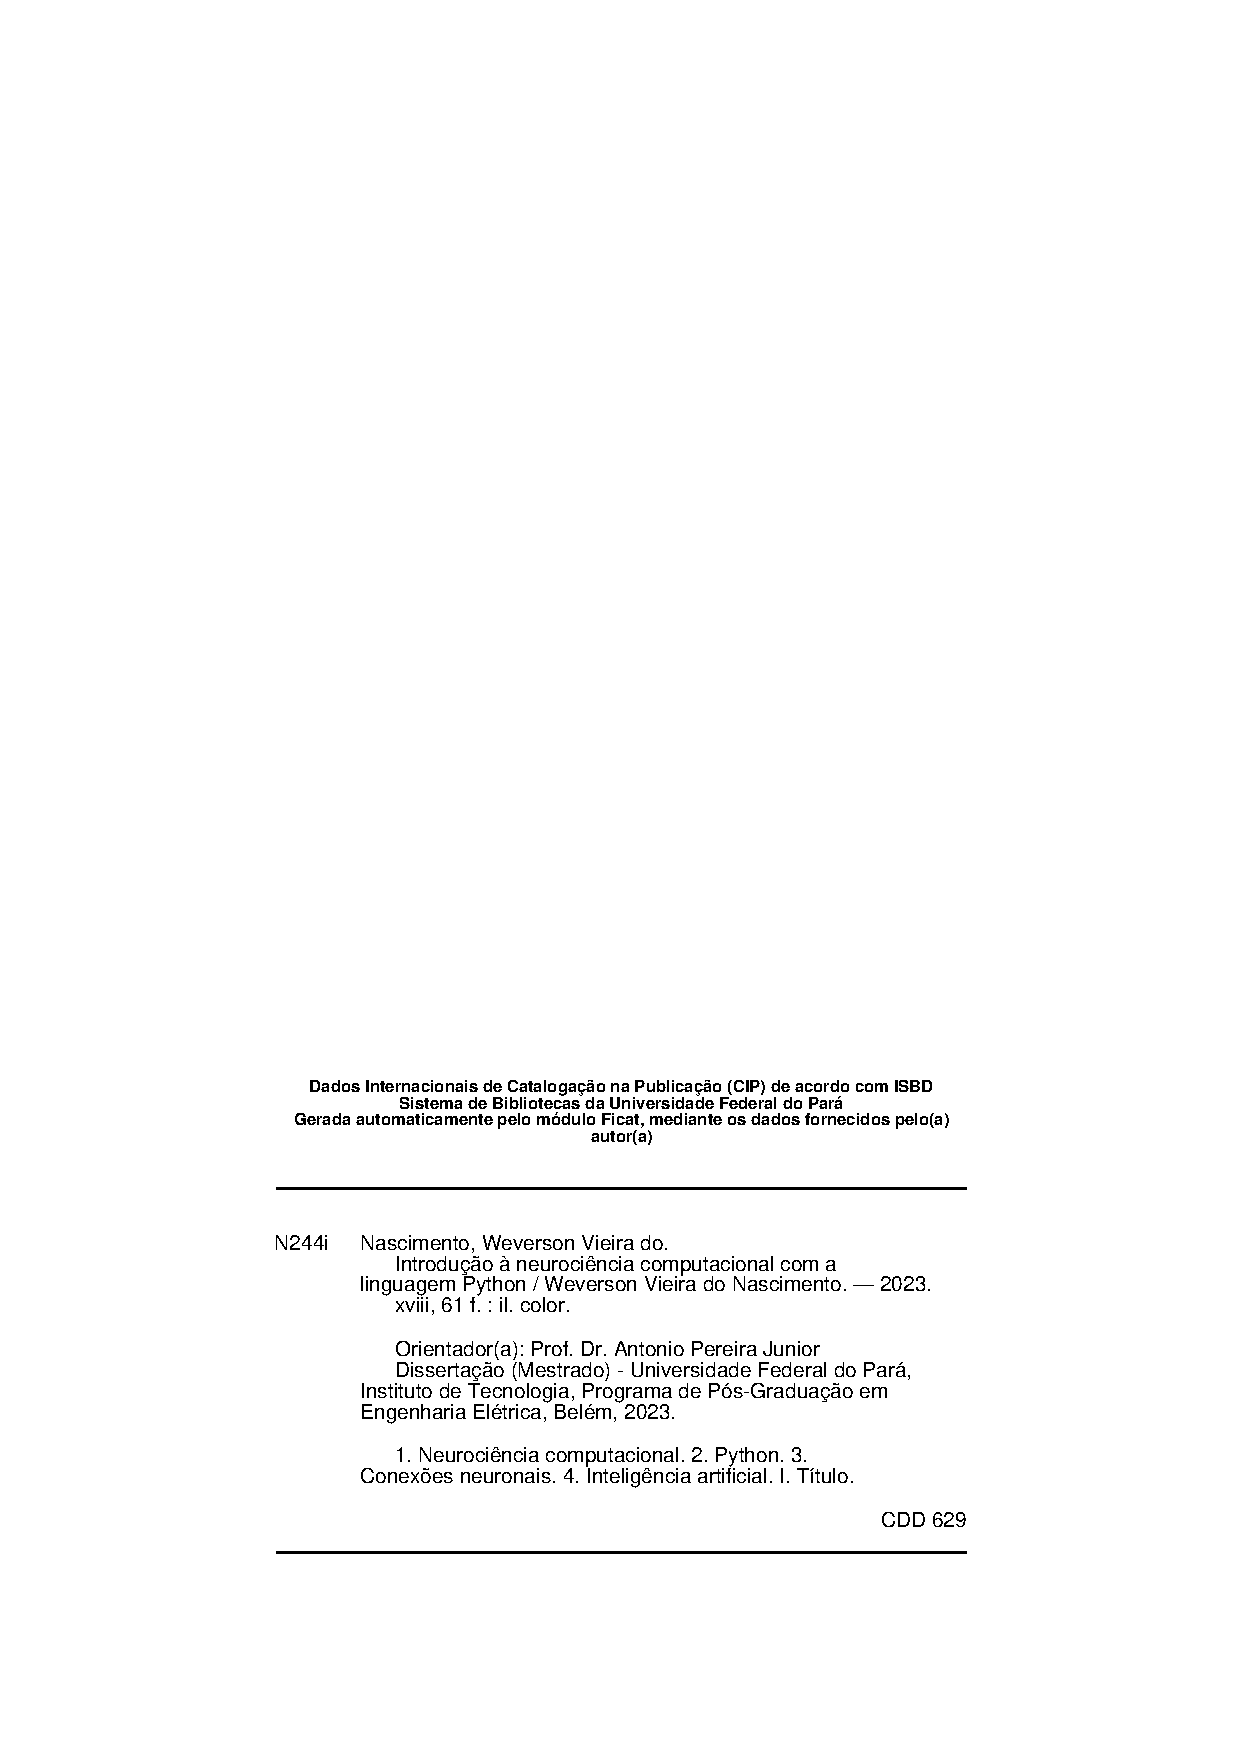
\includepdf{modelo-ufpa/ficha.pdf}
% \end{fichacatalografica}
\newpage
\begin{fichacatalografica}
	\imprimirfichacatalografica
\end{fichacatalografica}

% ---
% Inserir folha de aprovação (obrigatório)
% ---
% na versão final deve-se incluir a folha assinada
% \includepdf{folhadeaprovacao_final.pdf}
\begin{folhadeaprovacao}
	\ufpaPaginaDeAprovacao
    %\imprimirfolhadeaprovacao
\end{folhadeaprovacao}
% ---

% ---
% Dedicatória (opcional)
% ---
\begin{dedicatoria}
   \vspace*{\fill}
   \noindent
   \begin{flushright}
      \textit{escreva}\\
      \textit{aqui}\\
      \textit{a}\\
      \textit{dedicatória}
   \end{flushright}
\end{dedicatoria}
% ---

% ---
% Agradecimentos (opcional)
% ---
\begin{agradecimentos}
a escrever.
\end{agradecimentos}
% ---

% ---
% Epígrafe (opcional - NBR 10520)
% ---
\begin{epigrafe}
    \vspace*{\fill}
	\begin{flushright}
		\textit{``texto da epígrafe''\\
		autor}
	\end{flushright}
\end{epigrafe}
% ---

% ---
% RESUMOS
% ---
\setlength{\absparsep}{18pt}
\begin{resumo}
%O  resumo  deve  ressaltar  o  objetivo,  o  método,  os  resultados  e  as  conclusões  do  documento.  A  ordem  e  a  extensão destes itens dependem do tipo de resumo (informativo ou indicativo) e do tratamento que cada item recebe no documento original.
%O  resumo  deve  ser  composto  de  uma  sequência  de  frases  concisas,  afirmativas  e  não  de  enumeração  de  tópicos. Recomenda-se o uso de parágrafo único.
%A  primeira  frase  deve  ser  significativa,  explicando  o  tema  principal  do  documento.  A  seguir,  deve-se  indicar  a informação sobre a categoria do tratamento (memória, estudo de caso, análise da situação etc.).
texto do resumo

\textbf{Palavras-chave}: \imprimirpalavraschave
\end{resumo}

\begin{resumo}[Abstract]
 \begin{otherlanguage*}{english}
abstract

   \vspace{\onelineskip}
 
   \noindent 
   \textbf{Keywords}: escrever manualmente.
 \end{otherlanguage*}
\end{resumo}

% ---
% inserir lista de ilustrações (opcional)
% ---
\pdfbookmark[0]{\listfigurename}{lof}
\listoffigures*
\cleardoublepage
% ---

% ---
% inserir lista de quadros (não existe na norma, consta como ilustração)
% ---
%\pdfbookmark[0]{\listofquadrosname}{loq}
%\listofquadros*
%\cleardoublepage
% ---

% ---
% inserir lista de tabelas (opcional)
% ---
\pdfbookmark[0]{\listtablename}{lot}
\listoftables*
\cleardoublepage
% ---

% ---
% inserir lista de algoritmos (não consta na norma)
% ---
%\pdfbookmark[0]{\listalgorithmcfname}{loa}
%\imprimirlistadealgoritmos
%\cleardoublepage
% ---

% ---
% inserir lista de abreviaturas e siglas (opcional)
% ---
% listar em ordem alfabética
\begin{siglas}
\item[UFPA] Universidade Federal do Pará
\end{siglas}
% ---

% ---
% inserir lista de símbolos (opcional)
% ---
% inserir na ordem que aparecem no texto
\begin{simbolos}
\item[$\alpha$] Estrela de maior brilho de uma constelação % eu gosto de ver estrelas (literalmente)
\end{simbolos}
% ---

% ---
% inserir o sumario (obrigatório - NBR 6027)
% ---
\pdfbookmark[0]{\contentsname}{toc}
\tableofcontents*
\cleardoublepage
% ---



% ----------------------------------------------------------
% ELEMENTOS TEXTUAIS
% ----------------------------------------------------------
\textual

% ---
% algumas pessoas gostam de escrever os capítulos em .tex separados
% se for o caso eles devem ser incluídos no texto principal usando o comando abaixo.
% colocar tantos "includes" quantos forem os capítulos do texto.
% um inconveniente disso é não aparecer a estrutura de tópicos completa (pelo menos no overleaf);
% é possível colocando os \chapter no main, e manter o restante nos .tex separados,
% mas as seções ainda ficariam separadas, e o include, por padrão, gera uma nova página, o que
% pode ser complicado de lidar
% ---
\chapter{Introdução}\label{cap:introducao}
\section{Contexto}

\section{Justificativa}

\section{Objetivos}
\subsection{Objetivo Geral}
Elaborar um roteiro para execução de um curso introdutório em neurociências computacionais usando linguagens de programação livres

\subsection{Objetivos Específicos}
\begin{itemize}
\item Obter uma bibliografia robusta para servir de base na elaboração do roteiro
\item Criar um conjunto de códigos contendo exemplos dos conceitos apresentados ao longo do roteiro
\item Consolidar o material criado em uma estrutura de fácil uso por interessados no tema em questão
\end{itemize}

\section{Metodologia}

\section{Estrutura do Trabalho}
O trabalho está estruturado da seguinte maneira: o Capítulo~\ref{cap:teoria} mostra os elementos da base teórica apresentada. Uma breve apresentação de definições sobre fisiologia, equações diferenciais ordinárias, probabilidade, noções sobre algoritmos e linguagem de programação são mostradas. O Capítulo~\ref{cap:temas} contém os temas teóricos e práticos que constituem o roteiro em si. O Capítulo~\ref{cap:conclusoes} contém as conclusões acerca do trabalho e os desdobramentos possíveis para este.

\chapter{Desenvolvimento}\label{cap:estimacao_pose}
\section{Introdução}

\section{blah blah blah}

% ----------------------------------------------------------
% Considerações Finais
% ----------------------------------------------------------
\chapter{Considerações finais}\label{cap:conclusoes}
Este trabalho apresentou uma série de conteúdos para a execução de um curso introdutório de neurociência computacional, voltado para diversos públicos, servindo como um guia de execução. Baseado em algumas execuções do curso, uma possível sequência didática para o mesmo é mostrada na Tabela~\ref{tab:sequencia_didatica}.
\begin{table}[tb]
	\IBGEtab{
		\caption{Proposta de sequência didática}
		\label{tab:sequencia_didatica}
	}{
	\begin{tabular}{|c|c|p{8cm}|}
	\hline
	Número da aula & Tema & Conteúdo \\
	\hline
	1 & Apresentação da disciplina & Apresentação do estado da arte \\
	\hline
	2-4 & Introdução & Neurobiologia; equações diferenciais; introdução ao Python \\
	\hline
	5-9 & Modelos de neurônio de disparo & Modelos LIF, ELIF, AELIF, Izhikevich, Hodgkin-Huxley \\
	\hline
	10-17 & Conexões entre neurônios & Sinapses; Sinapses dinâmicas; Multi-estabilidade; Modelos de Wilson-Cowan; Aprendizado \\
	\hline
	18-21 & Inteligência artificial & Redes neurai; Redes neuromórficas \\
	\hline
	22-24 & Conclusão & Apresentações/entregas de trabalhos; Avaliação da disciplina \\
	\hline
	\end{tabular}
}{
\fonte{o autor (\the\year)}
}
\end{table}
Também baseado em execuções do curso, foi elaborada a proposta de atividades avaliativas, referentes a cada capítulo apresentado, como segue:
\begin{alineas}
	\item Introdução: questões simples de neurobiologia, equações diferenciais e implementações de códigos em Python;
	\item modelos: alterações de parâmetros nos modelos LIF, ELIF e/ou AELIF;
	\item conexões: implementação de circuitos de multi-estabilidade com o modelo de Wilson-Cowan;
	\item tarefa final: implementação de codificação para a rede de disparo.
\end{alineas}

A proposta de execução do curso é utilizando o Google Colaboratory (Colab), que fornece um ambiente de programação em Python gratuito, incluindo recursos de \textit{hardware} robustos para aplicações de aprendizado de máquina.
%TODO: citação bisong google colaboratory
Como exibido na Figura~\ref{fig:colab}, o Colab é executado a partir de um \textit{Notebook}, que facilita a execução e reprodução de códigos e conteúdos em conjunto.
%TODO: citação interactive
Todos os códigos-fonte utilizados durante o curso, incluindo os que geram algumas das imagens deste texto, estão disponíveis em repositório online\footnote{\url{https://gitlab.com/weversonvn/intro_neurocomp}}, de maneira gratuita e com uma licença permissiva livre para uso.
\begin{figure}[tb]
	\centering
	\caption[Ambiente do Google Colaboratory com o conteúdo de neurônios de disparo]{Ambiente do Google Colaboratory com o conteúdo de neurônios de disparo}
	\label{fig:colab}
	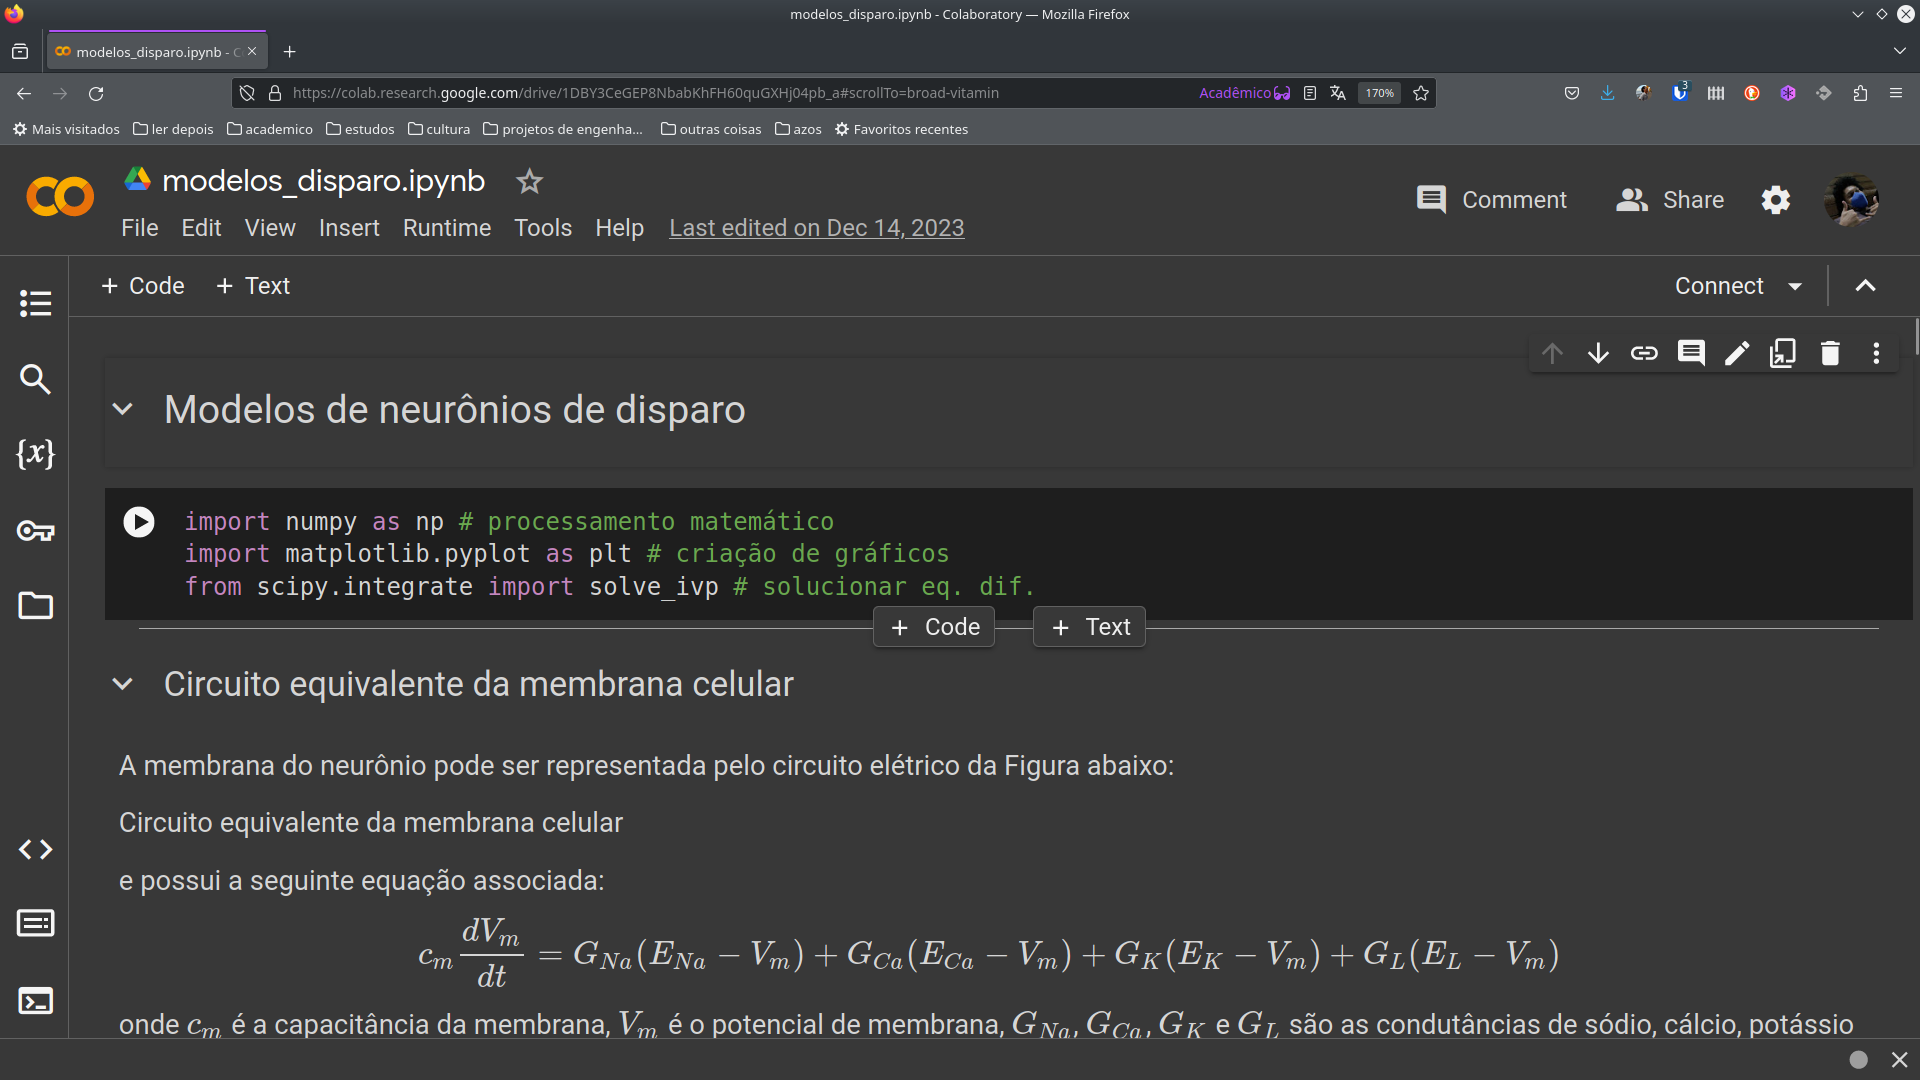
\includegraphics[width=0.7\linewidth]{figs/colab}
	\legend{Fonte: o autor (\the\year)}
\end{figure}

Possíveis melhorias para o curso começam pelo refinamento dos conteúdos já existentes, baseado nas considerações que venham a ser obtidas por eventuais alunos que o façam, como a alteração da ordem dos conteúdos, maior detalhamento de algum tópico específico, diminuição de outros. Além disso, um material voltado para exercícios pode ser bastante útil, tanto dos conteúdos teóricos quanto dos práticos, com destaque para tarefas em Python voltadas para cursos onde o público alvo não tem grande familiaridade com a linguagem ou com programação.

Como conteúdos novos pode-se incluir a simulação de modelos multi-compartimento, com destaque para a estimulação elétrica axonal, para estudar a propagação do potencial de ação ao longo do axônio.
%TODO: citação rattay a model
Outra possibilidade é a análise de sinais de eletroencefalograma (EEG), que são respostas elétricas obtidas das atividades cerebrais, podendo ser utilizadas para associações com comorbidades, como depressão e ansiedade.
%TODO: cavanagh multiple
Por fim, a apresentação de pacotes do Python voltados para análises semelhantes às apresentadas no curso pode ser incluído, uma vez que o uso destes potencialmente se torna mais simplificado com o entendimento obtido a partir do conteúdo deste trabalho.

% ---

% ----------------------------------------------------------
% ELEMENTOS PÓS-TEXTUAIS
% ----------------------------------------------------------
\postextual
% ----------------------------------------------------------

% ----------------------------------------------------------
% Referências bibliográficas (obrigatório - NBR 6023)
% ----------------------------------------------------------
% Os elementos essenciais são: autor(es), título, edição, local, editora e data de publicação
%  Quando se tratar de obras consultadas online,  também  são  essenciais  as  informações  sobre  o  endereço  eletrônico, apresentado  entre  os  sinais  <  >,  precedido  da  expressão  Disponível  em:  e  a  data  de  acesso  ao  documento,  precedida  da expressão Acesso em:, opcionalmente acrescida dos dados referentes a hora, minutos e segundos

% o template já faz no formato adequado
% eu fiz um arquivo .bib separado que é importado aqui
\bibliography{neurocomp}
% ---

% antes do apêndices um item opcional é o glossário
% se incluído é em ordem alfabética

% ----------------------------------------------------------
% Apêndices (opcional)
% ----------------------------------------------------------

% ---
% Inicia os apêndices
% ---
%\begin{apendicesenv}
	
	% Imprime uma página indicando o início dos apêndices
	% a norma não diz para criar essa página
%	\partapendices

% usar um include com \chapter para cada apêndice
	
%\end{apendicesenv}
% ---

% ----------------------------------------------------------
% Anexos (opcional)
% ----------------------------------------------------------

% ---
% Inicia os anexos
% ---
%\begin{anexosenv}
	
	% Imprime uma página indicando o início dos anexos
	% novamente a norma não diz para criar essa página
%	\partanexos

% novamente usar um include com \chapter para cada anexo
% ou usar \includepdf caso seja documento externo (o mais provável no caso de anexo)
	
%\end{anexosenv}

% o último item opcional é o índice
% se incluído é conforme a NBR 6034

\end{document}
